\documentclass{article}  %book report 
\usepackage{ctex}
\usepackage{graphicx}
\title{第一个中文文件}
\author{\kaishu AlimyBreak}
\date{\today}



\begin{document}

\maketitle
\tableofcontents

\section{空白符号}
%空行分段,多个空行等同1个
%自动缩进,绝对不能使用空格代替
%英文中多个空格处理成1个空格,中文中空格将被忽略(阿拉伯数字算英文字符)
%中英文混合时,中英文之间会自动加一个空格(XeLatex处理)
%禁止使用中文全角空格
% \quad 产生一个1em的空白
% \qquad 2em
% \thinspace 1/6em
% \enspace 0.5em
% 硬空格 a~b
% \kern 1pc 
% \hspace{35pt}
% 
1 2

2

中文   空格

中文\ \ 空desfsg格

abcde\quad 这里\quad 是正文

abcde\qquad 这里\qquad 是正文

abcde\thinspace 这里\thinspace 是正文

abcde\enspace 这里\enspace 是正文

a~b

a \kern 1pc b 

a \kern -1pc b 


a \hspace{35pt} n

a \hfill n

\section{\LaTeX 控制符}
\# \$ \% \{ \} \~ \textbackslash \\\\

\section{排版符号}
\S \P \dag \ddag \copyright \pounds


\TeX{dada}


\section{插入图片}
\graphicspath{{figure/}}
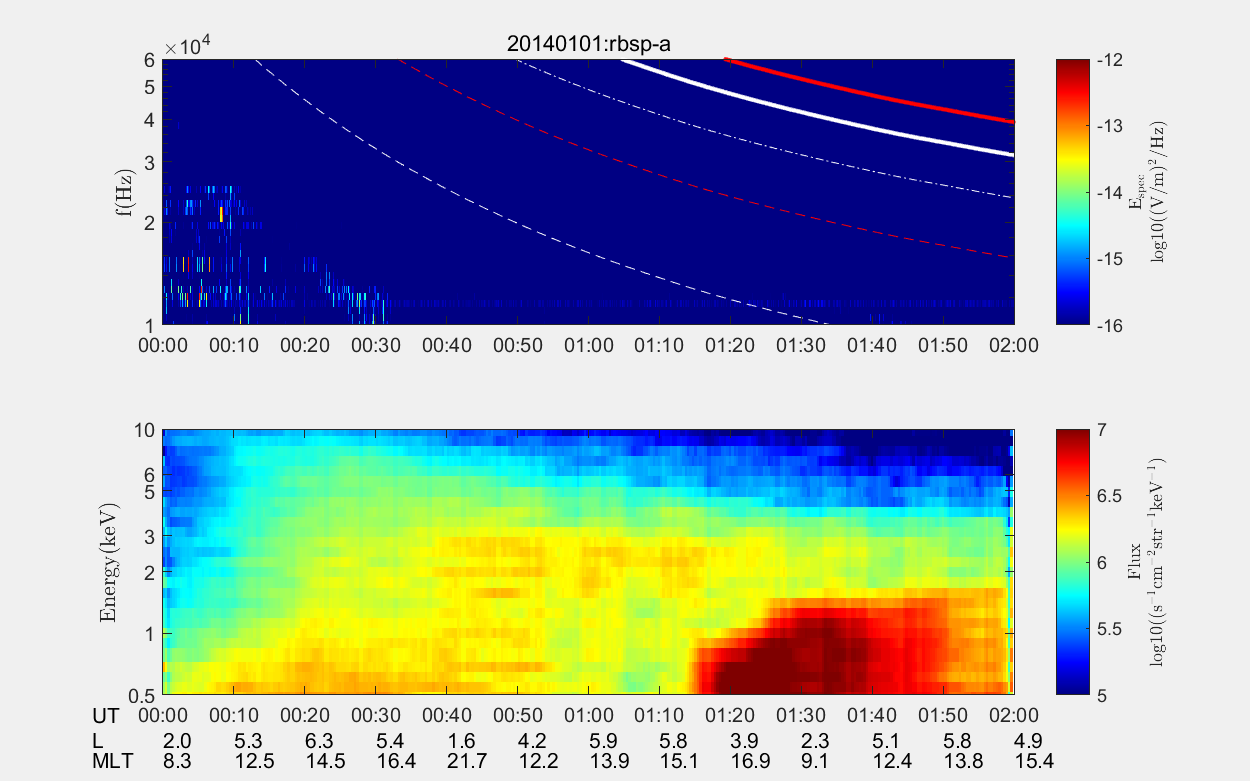
\includegraphics[scale=0.5]{rbsp-a20140101T000000.png}

\section{表格}
\begin{tabular}{l  c  c  c  r}
姓名 & 语文 & 数学 & 外语 & 备注 \\
\hline
qq & 18 & 12 & 23 & 不及格


\end{tabular}

\end{document}